\subsection{Recurrent neural networks}\label{sec:RNN}
%\cm{Mention that RNN is cyclic graph.}
Recurrent neural nets (RNNs) are another family of powerful models, which are designed to process time series data and other sequence data. RNNs have successful applications in speech recognition \citep{sak2014long}, machine translation \citep{wu2016google}, genome sequencing \citep{cao2018deep}, etc. The structure of an RNN naturally forms a computational graph, and can be easily combined with other structures such as CNNs to build large computational graph models for complex tasks. Here we introduce vanilla RNNs and improved variants such as long short-term memory (LSTM).

%\begin{figure}
%\centering
%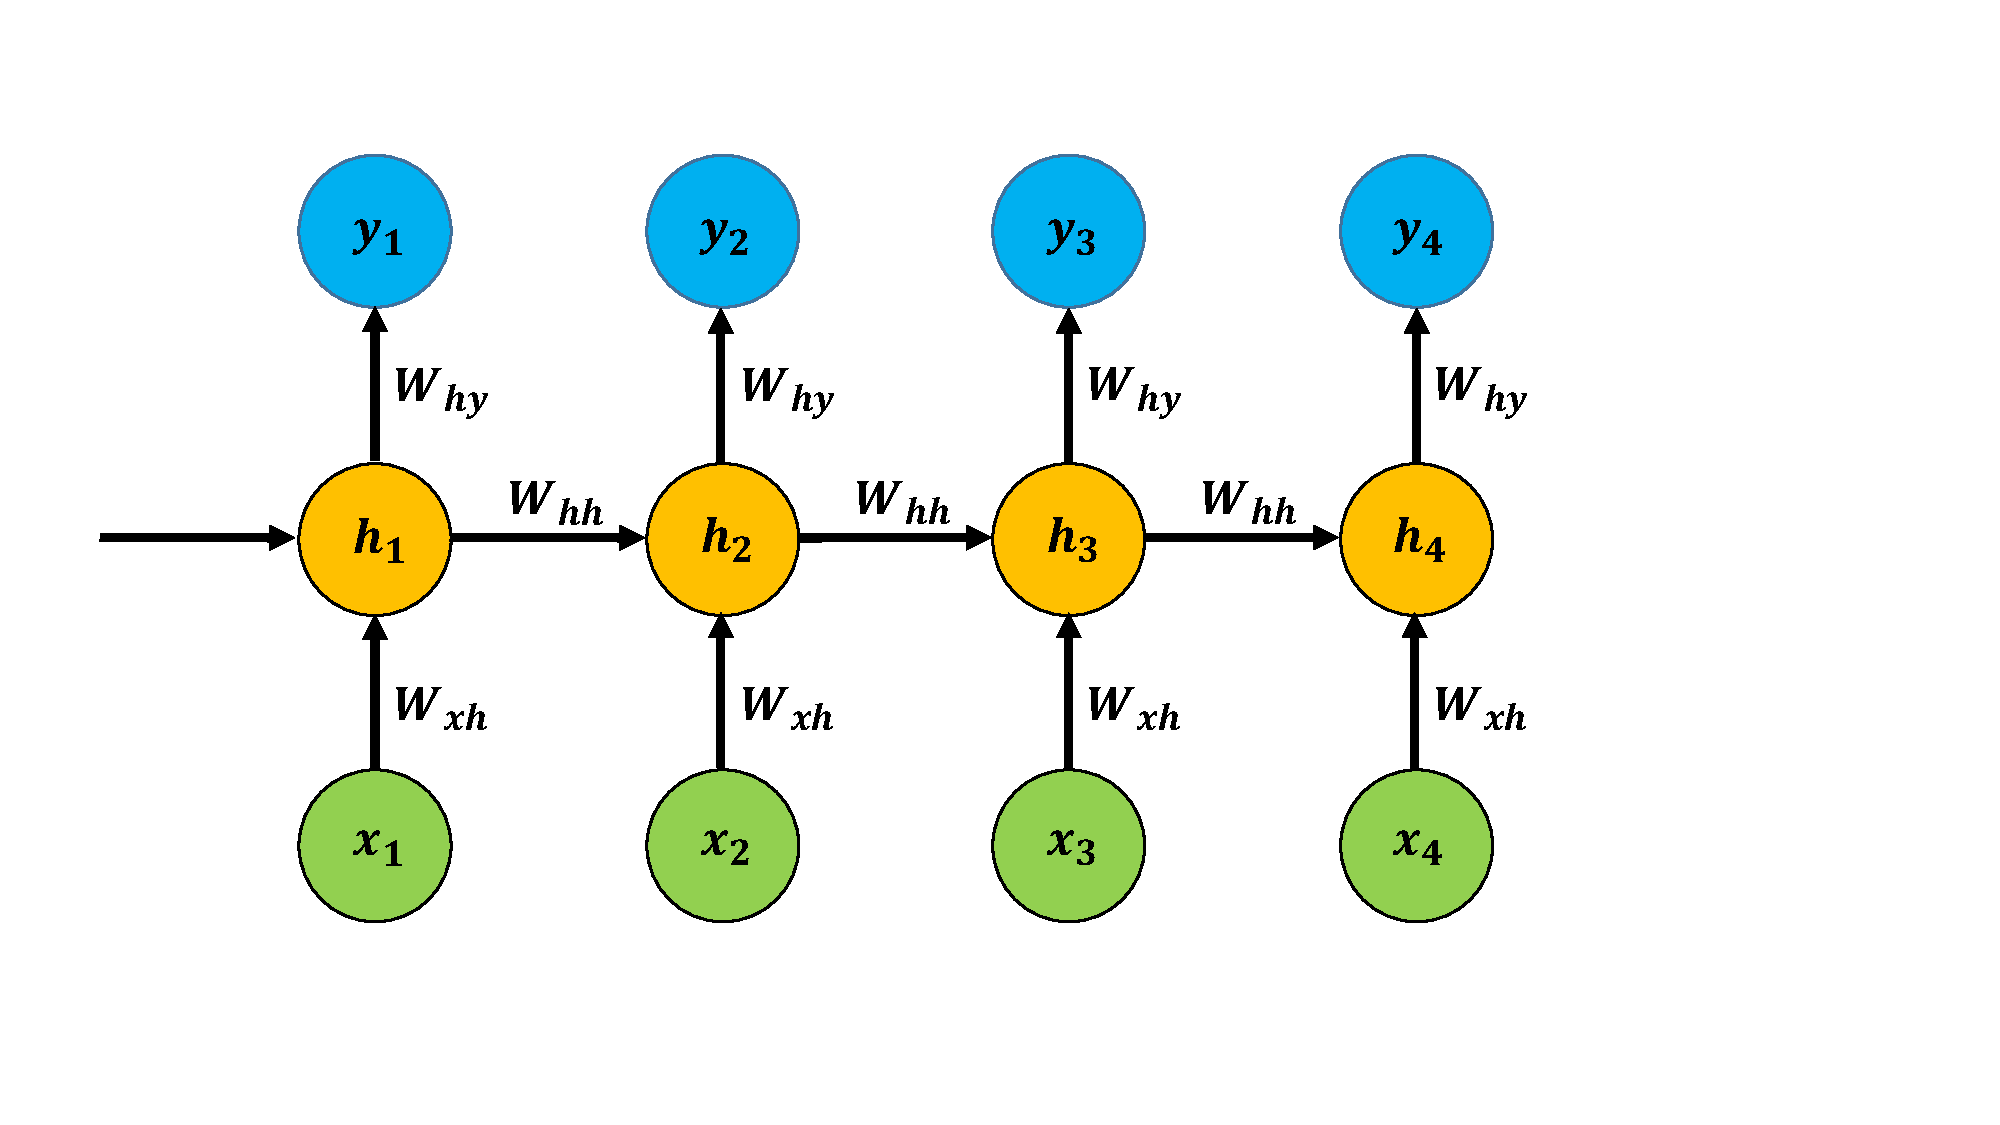
\includegraphics[width = 0.65\textwidth]{Figure/RNN1}
%\caption{A vanilla RNN with one hidden layer. Top row is outputs, middle row is hidden states, and bottom row is inputs. Parameters are shared across time.} \label{fig:RNN1}
%\end{figure}
%\begin{figure}\label{fig:RNN1}
%\centering
%\begin{subfigure}[b]{0.3\textwidth}
%\centering
%        \includegraphics[width = 0.95\textwidth]{Figure/RNN1-1}
%\end{subfigure}
%\begin{subfigure}[b]{0.3\textwidth}
%\centering
%        \includegraphics[width = 0.95\textwidth]{Figure/RNN1-2}
%\end{subfigure}
%\begin{subfigure}[b]{0.3\textwidth}
%\centering
%        \includegraphics[width = 0.95\textwidth]{Figure/RNN1-3}
%\end{subfigure}
%\caption{Vanilla RNNs with different inputs/outputs settings. \textbf{Left} has one input but multiple outputs. \textbf{Middle} has multiple inputs but one output. \textbf{Right} has multiple inputs and outputs. Parameters are shared across time.}
%\end{figure}

\begin{figure}
\centering
\begin{tabular}{ccc}
\includegraphics[width = 0.3\textwidth]{RNN1-1} & \includegraphics[width = 0.3\textwidth]{RNN1-2} & \includegraphics[width = 0.3\textwidth]{RNN1-3} \tabularnewline
(a) One-to-many & (b) Many-to-one & (c) Many-to-many
\end{tabular}
\caption{Vanilla RNNs with different inputs/outputs settings. (a) has one input but multiple outputs; (b) has multiple inputs but one output; (c) has multiple inputs and outputs. Note that the parameters are shared across time steps.}\label{fig:RNN1}
\end{figure}

\subsubsection{Vanilla RNNs}
Suppose we have general time series inputs $\xx_1,\xx_2,\ldots,\xx_T$. A vanilla RNN models the ``hidden state'' at time $t$ by a vector $\hh_t$, which is subject to the recursive formula
\begin{equation}\label{eq:recur}
\hh_t  = \ff_{\btheta}(\hh_{t-1}, \xx_t).
\end{equation}
Here, $f_{\btheta}$ is generally a nonlinear function parametrized by $\btheta$. Concretely, a vanilla RNN with one hidden layer has the following form\footnote{Similar to the activation function $\bsigma(\cdot)$, the function $\btanh(\cdot)$ means element-wise operations.}
\begin{align*}
\hh_t  &= \btanh\left( \bW_{hh} \hh_{t-1}+ \bW_{xh} \xx_t + \bb_\hh \right), \qquad \text{where}~ \tanh(a) = \tfrac{e^{2a} - 1}{e^{2a} + 1}, \\
\zz_t &= \bsigma \left(\bW_{hy} \hh_t + \bb_\zz \right),
\end{align*}
where $\bW_{hh}, \bW_{xh}, \bW_{hy}$ are trainable weight matrices, $\bb_\hh, \bb_\zz$ are trainable bias vectors, and $\zz_t$ is the output at time $t$. Like many classical time series models, those parameters are shared across time. Note that in different applications, we may have different input/output settings (cf.~Figure~\ref{fig:RNN1}). Examples include
\begin{itemize}
\item{ \textbf{One-to-many:} a single input with multiple outputs; see Figure~\ref{fig:RNN1}(a). A typical application is image captioning, where the input is an image and outputs are a series of words.
}
\item{ \textbf{Many-to-one:} multiple inputs with a single output; see Figure~\ref{fig:RNN1}(b). One application is text sentiment classification, where the input is a series of words in a sentence and the output is a label (e.g., positive vs.~negative).
}
\item{ \textbf{Many-to-many:} multiple inputs and outputs; see Figure~\ref{fig:RNN1}(c). This is adopted in machine translation, where inputs are words of a source language (say Chinese) and outputs are words of a target language (say English).
}
\end{itemize}

As the case with feed-forward neural nets, we minimize a loss function using back-propagation, where the loss is typically
\begin{equation*}
\ell_{\cT}(\btheta) = \sum_{t \in \cT} \cL(y_t, \zz_t) = - \sum_{t \in \cT} \sum_{k=1}^K \bbone\{y_t = k\} \log \left( \frac{\exp([\zz_t]_k)}{\sum_k \exp([\zz_t]_k)} \right),
\end{equation*}
where $K$ is the number of categories for classification (e.g., size of the vocabulary in machine translation), and $\cT \subset [T]$ is the length of the output sequence. During the training, the gradients $\partial \ell_{\cT} / \partial \hh_t$ are computed in the reverse time order (from $T$ to $t$). For this reason, the training process is often called \textit{back-propagation through time}. 

One notable drawback of vanilla RNNs is that, they have difficulty in capturing long-range dependencies in sequence data when the length of the sequence is large. This is sometimes due to the phenomenon of \emph{exploding$\,$/$\,$vanishing gradients}. Take Figure~\ref{fig:RNN1}(c) as an example. Computing $\partial \ell_{\cT} / \partial \hh_1$ involves the product $\prod_{t=1}^3 (\partial \hh_{t+1} / \partial \hh_{t})$ by the chain rule. However, if the sequence is long, the product will be the multiplication of many Jacobian matrices, which usually results in exponentially large or small singular values. To alleviate this issue, in practice, the forward pass and backward pass are implemented in a shorter sliding window $\{t_1, t_1+1, \ldots,t_2\}$, instead of the full sequence $\{1,2,\ldots, T\}$. Though effective in some cases, this technique alone does not fully address the issue of long-term dependency. 

\subsubsection{GRUs and LSTM} There are two improved variants that alleviate the above issue: gated recurrent units (GRUs) \citep{cho2014learning} and long short-term memory (LSTM) \citep{hochreiter1997long}.
\begin{itemize}
\item{ A \textbf{GRU} refines the recursive formula \eqref{eq:recur} by introducing \textit{gates}, which are vectors of the same length as $\hh_t$. The gates, which take values in $[0,1]$ elementwise, multiply with $\hh_{t-1}$ elementwise and determine how much they keep the old hidden states.
}
\item{ An \textbf{LSTM} similarly uses gates in the recursive formula. In addition to $\hh_t$, an LSTM maintains a \textit{cell state}, which takes values in $\mathbb{R}$ elementwise and are analogous to counters.
}
\end{itemize}
Here we only discuss LSTM in detail. Denote by $\odot$ the element-wise multiplication. We have a recursive formula in replace of \eqref{eq:recur}:
\begin{align*}
\left( \begin{array}{c} \ii_t \\ \ff_t \\ \oo_t \\ \bgg_t \end{array} \right) &= \left( \begin{array}{c} \bsigma \\ \bsigma \\ \bsigma \\ \btanh \end{array} \right) \bW \left( \begin{array}{c} \hh_{t-1} \\ \xx_t \\ 1 \end{array} \right), \\
\cc_t &= \ff_t \odot \cc_{t-1} + \ii_t \odot \bgg_t, \\
\hh_t &= \oo_t \odot \btanh(\cc_t),
\end{align*}
where $\bW$ is a big weight matrix with appropriate dimensions. The cell state vector $\cc_t$ carries information of the sequence (e.g., singular/plural form in a sentence). The forget gate $\ff_t$ determines how much the values of $\cc_{t-1}$ are kept for time $t$, the input gate $\ii_t$ controls the amount of update to the cell state, and the output gate $\oo_t$ gives how much $\cc_t$ reveals to $\hh_t$.  Ideally, the elements of these gates have nearly binary values. For example, an element of $\ff_t$ being close to $1$ may suggest the presence of a feature in the sequence data. Similar to the skip connections in residual nets, the cell state $\cc_t$ has an additive recursive formula, which helps back-propagation and thus captures long-range dependencies.

\begin{figure}
\centering
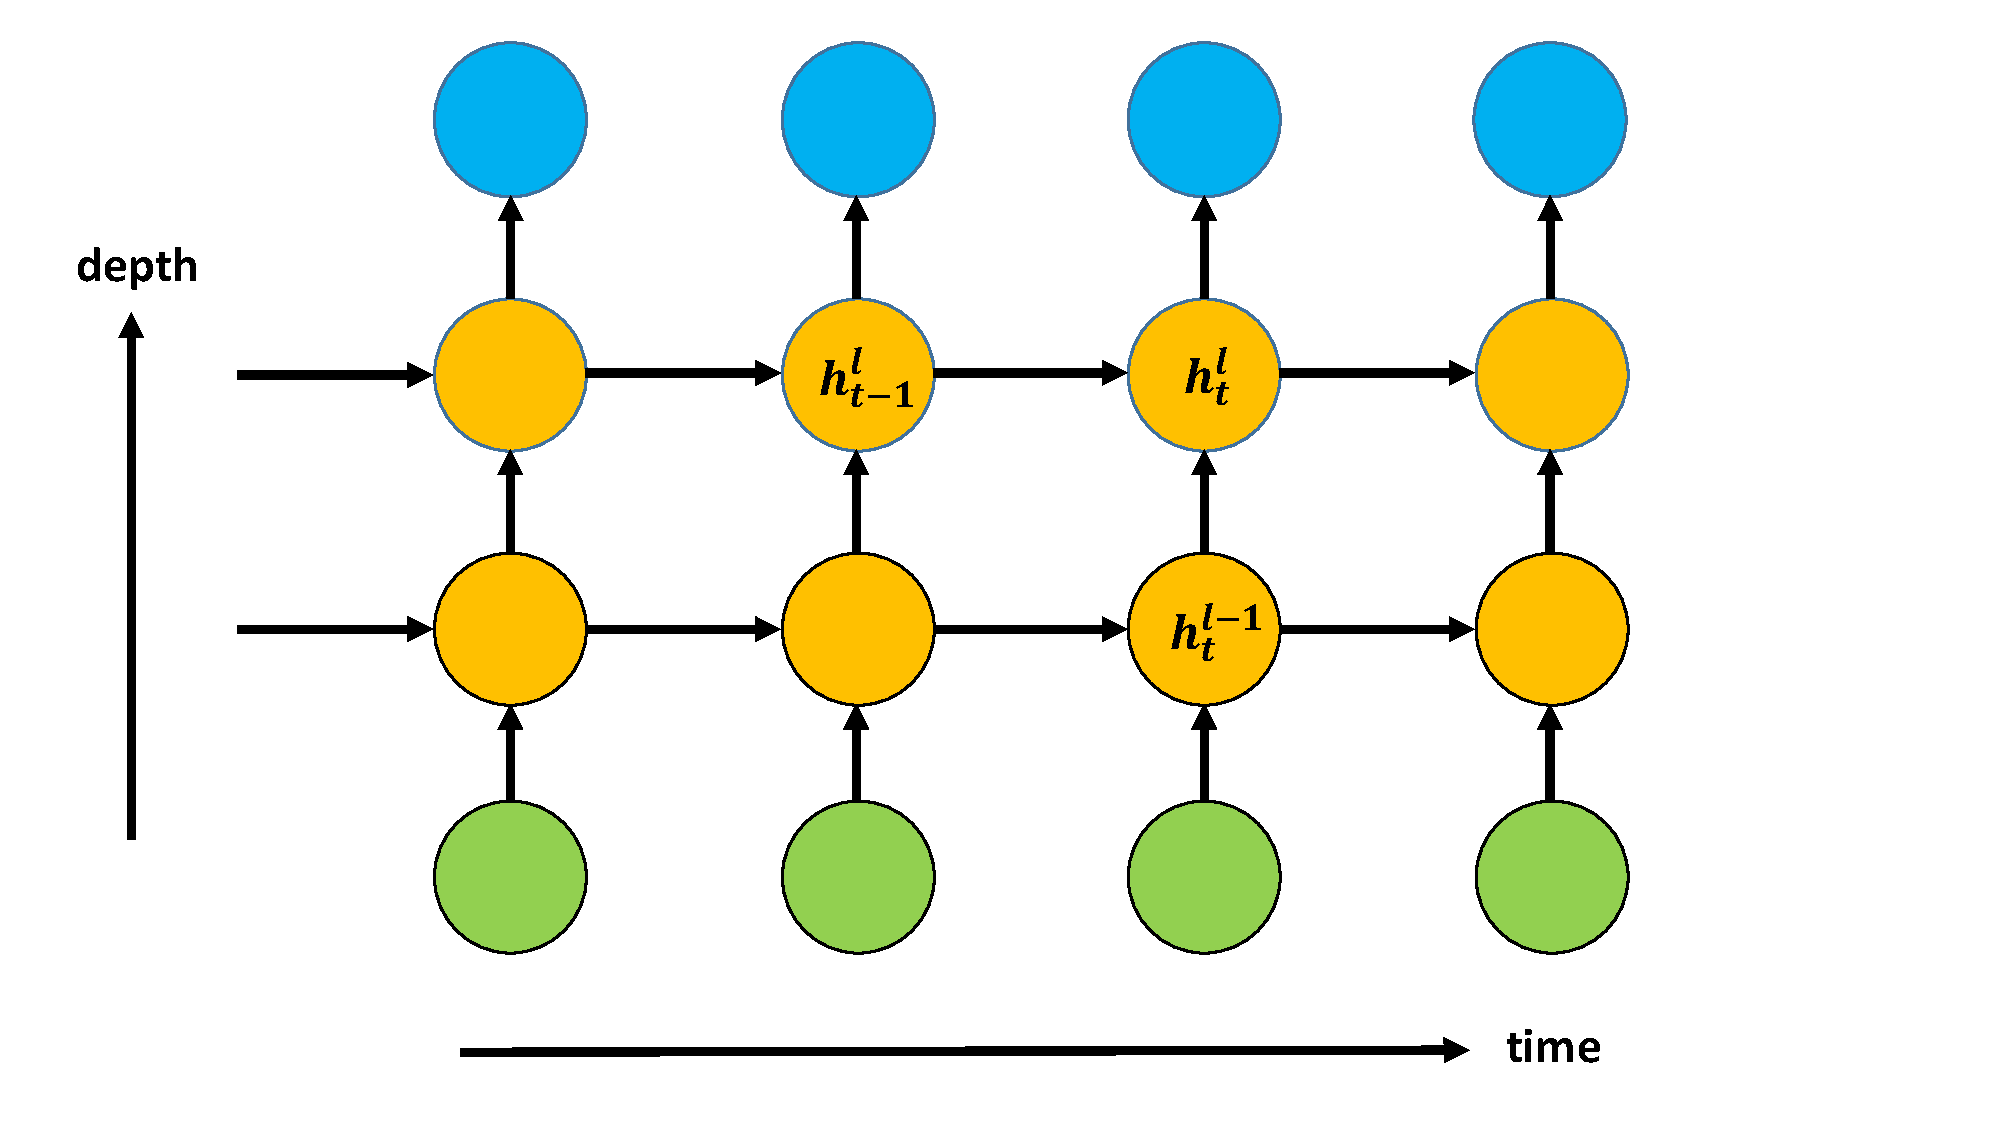
\includegraphics[width = 0.4\textwidth]{RNN2}
\caption{A vanilla RNN with two hidden layers. Higher-level hidden states $\hh_t^{\ell}$ are determined by the old states $\hh_{t-1}^\ell$ and lower-level hidden states $\hh_t^{\ell-1}$. Multilayer RNNs generalize both feed-forward neural nets and one-hidden-layer RNNs.}\label{fig:RNN2}
\end{figure}

\subsubsection{Multilayer RNNs} Multilayer RNNs are generalization of the one-hidden-layer RNN discussed above. Figure~\ref{fig:RNN2} shows a vanilla RNN with two hidden layers. In place of \eqref{eq:recur}, the recursive formula for an RNN with $L$ hidden layers now reads
\begin{equation*}
\hh_t^{\ell} =  \btanh \left[\bW^\ell \left( \begin{array}{c} \hh_t^{\ell-1} \\ \hh_{t-1}^\ell \\ 1 \end{array} \right) \right], \quad \text{for all}\, \ell \in [L], \qquad \hh_t^{0} \triangleq \xx_t.
\end{equation*}
Note that a multilayer RNN has two dimensions: the sequence length $T$ and depth $L$. Two special cases are the feed-forward neural nets (where $T=1$) introduced in Section~\ref{sec:super}, and RNNs with one hidden layer (where $L=1$). Multilayer RNNs usually do not have very large depth (e.g., $2$--$5$), since $T$ is already very large.

Finally, we remark that CNNs, RNNs, and other neural nets can be easily combined to tackle tasks that involve different sources of input data. For example, in image captioning, the images are first processed through a CNN, and then the high-level features are fed into an RNN as inputs. Theses neural nets combined together form a large computational graph, so they can be trained using back-propagation. This generic training method provides much flexibility in various applications.
